%%%%%%%%%%%%%%%%%%%%%%%%%%%%%%%%%%%%%%%%%
% Beamer Presentation
% LaTeX Template
% Version 1.0 (10/11/12)
%
% This template has been downloaded from:
% http://www.LaTeXTemplates.com
%
% License:
% CC BY-NC-SA 3.0 (http://creativecommons.org/licenses/by-nc-sa/3.0/)
%
%%%%%%%%%%%%%%%%%%%%%%%%%%%%%%%%%%%%%%%%%

%----------------------------------------------------------------------------------------
%	PACKAGES AND THEMES
%----------------------------------------------------------------------------------------

\documentclass[xcolor=dvipsnames, allowframebreaks, 14pt]{beamer}

\mode<presentation> {
\definecolor{darkred}{RGB}{164,56,56}
\definecolor{lightred}{RGB}{200,100,100}
% The Beamer class comes with a number of default slide themes
% which change the colors and layouts of slides. Below this is a list
% of all the themes, uncomment each in turn to see what they look like.

%\usetheme{default}
%\usetheme{AnnArbor}
%\usetheme{Antibes}
%\usetheme{Bergen}
%\usetheme{Berkeley}
%\usetheme{Berlin}
%\usetheme{Boadilla}
%\usetheme{CambridgeUS}
%\usetheme{Copenhagen}
%\usetheme{Darmstadt}
%\usetheme{Dresden}
%\usetheme{Frankfurt}
%\usetheme{Goettingen}
%\usetheme{Hannover}
%\usetheme{Ilmenau}
%\usetheme{JuanLesPins}
%\usetheme{Luebeck}
%\usetheme{Madrid}
%\usetheme{Malmoe}
%\usetheme{Marburg}
%\usetheme{Montpellier}
%\usetheme{PaloAlto}
%\usetheme{Pittsburgh}
\usetheme{Rochester}
%\usetheme{Singapore}
%\usetheme{Szeged}
%\usetheme{Warsaw}

% As well as themes, the Beamer class has a number of color themes
% for any slide theme. Uncomment each of these in turn to see how it
% changes the colors of your current slide theme.

%\usecolortheme{albatross}
%\usecolortheme{beaver}
%\usecolortheme{beetle}
%\usecolortheme{crane}
%\usecolortheme{dolphin}
%\usecolortheme{dove}
%\usecolortheme{fly}
%\usecolortheme{lily}
%\usecolortheme{orchid}
%\usecolortheme{rose}
%\usecolortheme{seagull}
%\usecolortheme{seahorse}
%\usecolortheme{whale}
%\usecolortheme{wolverine}
%\setbeamertemplate{footline} % To remove the footer line in all slides uncomment this line
\setbeamertemplate{footline}[frame number] % To replace the footer line in all slides with a simple slide count uncomment this line
\setbeamertemplate{navigation symbols}{} % To remove the navigation symbols from the bottom of all slides uncomment this line 
\setbeamertemplate{title page}
{
    \begin{center}
    \Large\color{darkred}\inserttitle
    \end{center}
}
\usecolortheme[named=lightred]{structure}
\usefonttheme{professionalfonts}
\setbeamertemplate{frametitle continuation}{}
\setbeamercolor{frametitle}{bg=lightred}
\setbeamercolor{caption name}{fg=darkred}
}

\usepackage[french]{babel}
\usepackage{xcolor}
\usepackage{booktabs} % Allows the use of \toprule, \midrule and \bottomrule in tables
\usepackage{pgfplots}
\usepackage{tcolorbox}
\pgfplotsset{compat=1.15}
\usetikzlibrary{arrows}
\usetikzlibrary{patterns}
\usepackage{pstricks-add}
\usetikzlibrary{arrows,shapes,positioning,shadows,trees}
\usepackage{hyperref}
\hypersetup{
    colorlinks,
    citecolor=black,
    filecolor=black,
    linkcolor=black,
    urlcolor=black
}
\newcommand{\notimplies}{%
    \mathrel{{\ooalign{\hidewidth$\not\phantom{=}$\hidewidth\cr$\implies$}}}}
%\DeclareMathAlphabet\mathzapf{T1}{pzc}{mb}{it}
\usepackage{amsmath,wasysym}
\usepackage{latexsym}
\usepackage{mathrsfs}
\usepackage{amssymb}
\usepackage{wrapfig}
\bibliographystyle{amsplain}
\usepackage{systeme}
\usepackage{pdfpages}
\usepackage{graphicx}
\usepackage{caption}
\usetikzlibrary{calc}
\usetikzlibrary{babel}
\usepackage[european, straight voltages]{circuitikz}
\usepackage[T2A]{fontenc}

\AtBeginDocument{\centering}
\begin{document}

\tikzstyle{weight} = [font=\scriptsize]

\setlength{\parskip}{1ex}

\begin{frame}
\title{\Huge Électricité}
\titlepage\par\vspace{1ex}
\normalsize\color{black}Jonas Daverio
\end{frame}

\begin{frame}
\title{Principes physiques et premiers circuits}
\titlepage
\end{frame}

\begin{frame}{La charge électrique}

\only<2>{Unité : coulomb [$\si{\coulomb}$]}

\only<3>{
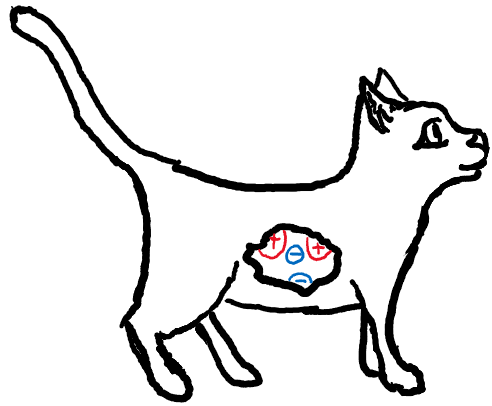
\includegraphics[height=0.5\textwidth]{Images/Chat neutre.png}
\par\captionof{figure}{Un chat électriquement neutre}}

\only<4>{
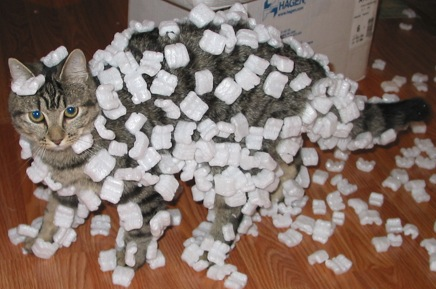
\includegraphics[height=0.5\textwidth]{Images/Chat statique.jpg}
\par\captionof{figure}{Un chat électriquement chargé}}

\end{frame}

\begin{frame}{Le courant électrique}

\only<2>{
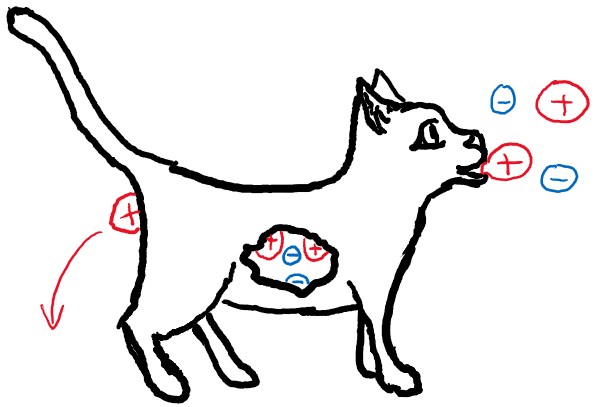
\includegraphics[height=0.5\textwidth]{Images/Chat-charge.png}
\par\captionof{figure}{Chat restant neutre lors de l'ingestion d'une charge}}

\only<3>{
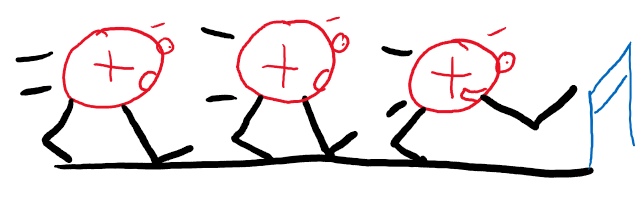
\includegraphics[width=0.9\textwidth]{Images/Course proton.png}
\par\captionof{figure}{Une course de charges (également nommée courant électrique)}}

\only<4,5>{
Unité : coulomb par seconde [$\si{\coulomb\per\second}$] \uncover<5>{ou ampère [$\si{\ampere}$]}
}
\end{frame}

\begin{frame}{La tension électrique}

\only<2>{
\begin{tabular}{*2{m{0.4\textwidth}}}
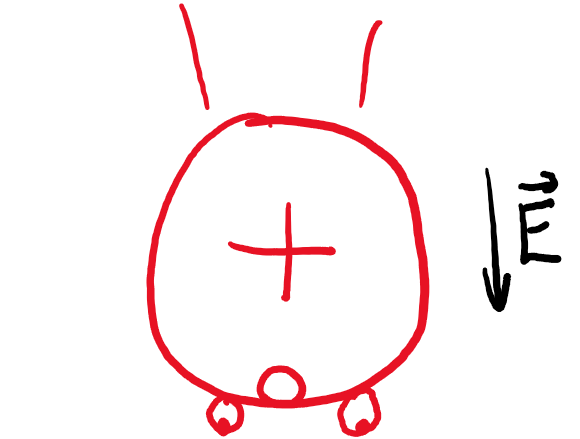
\includegraphics[width=0.4\textwidth]{Images/Charge accélérée.png}
\par Une charge dans un champ électrique
&
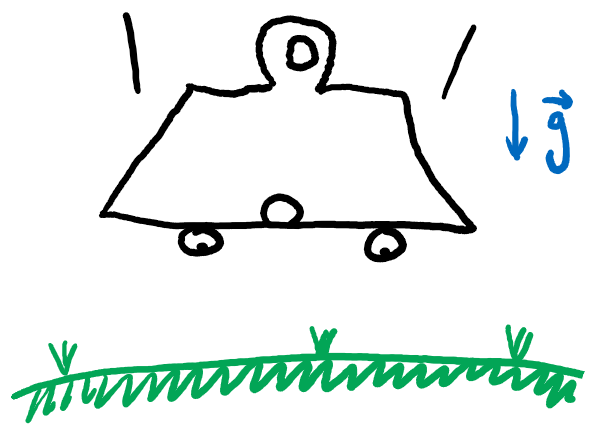
\includegraphics[width=0.4\textwidth]{Images/Masse accélérée.png}
\par Une masse dans un champ gravitationnel
\end{tabular}
}

\only<3,4>{
Unité : volt [$\si{\volt}$]} \uncover<4>{ou joule par coulomb [$\si{\joule\per\coulomb}$] \par Une énergie !}

\only<5>{Une force serait en newton par coulomb [$\si{\newton\per\coulomb}$]
\par C'est le champ électrique.}

\only<6>{L'énergie est plus utile.}

\end{frame}

\begin{frame}{Analogie hydraulique}

\only<2>{
\begin{tabular}{*2{p{0.4\textwidth}}}
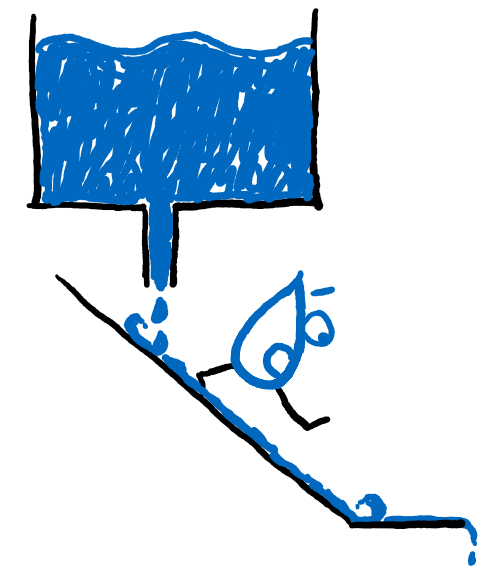
\includegraphics[height=0.45\textwidth]{Images/Goutte tombe.png}
\par Une goutte accélérée par une pente
&
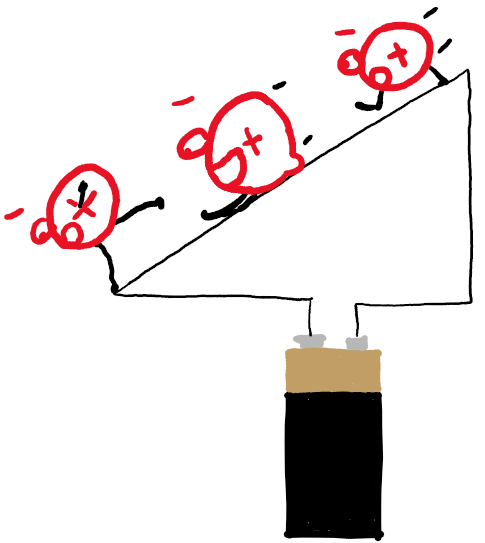
\includegraphics[height=0.45\textwidth]{Images/Charges tombent.png}
\par Des charges accélérées par une tension
\end{tabular}}

\only<3>{
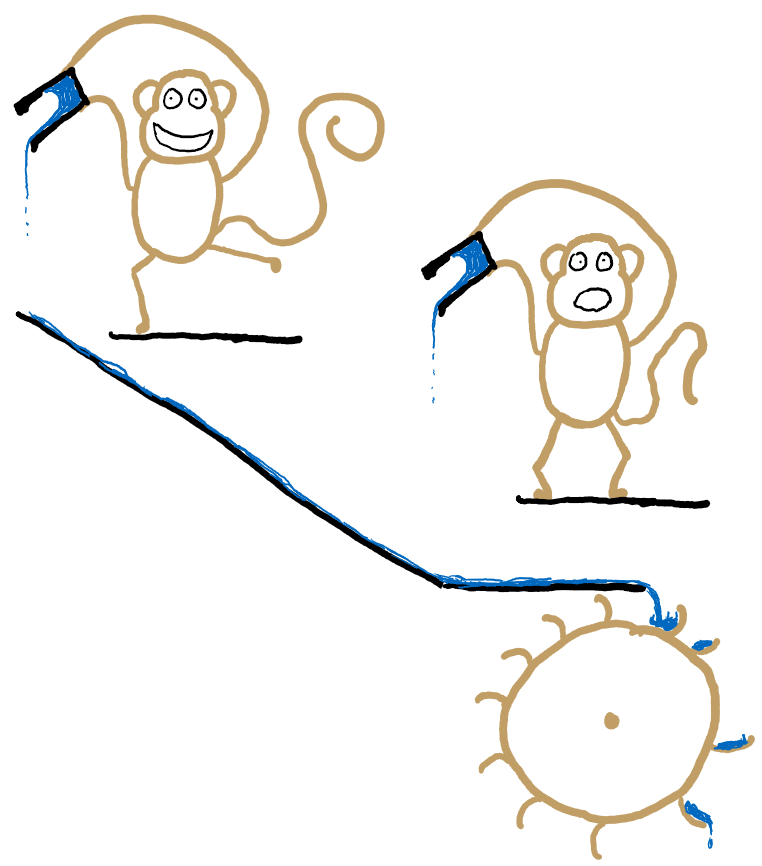
\includegraphics[height=0.55\textwidth]{Images/Hauteur eau.png}
\par\captionof{figure}{Deux bacs d'eau lancés de hauteurs différentes}}

\only<4>{
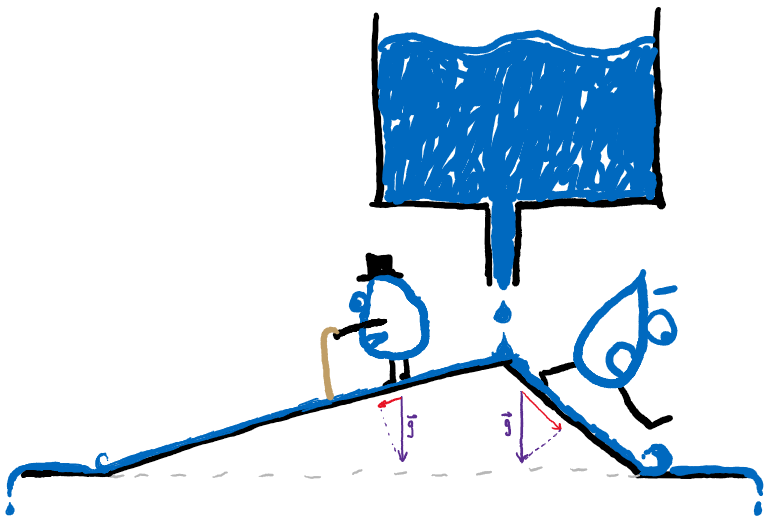
\includegraphics[height=0.5\textwidth]{Images/Deux pentes.png}
\par\captionof{figure}{Deux gouttes descendant des pentes différentes}}

\only<5>{C'est la hauteur qui compte, et donc l'énergie !}
    
\end{frame}

\begin{frame}
\title{Premiers circuits électriques et loi d'Ohm}
\titlepage
\end{frame}

\begin{frame}{Un premier exemple dégénéré}

\only<1>{
\begin{circuitikz}
\draw
    (0,0) to [V<=$U$] (0,4)
    to (3,4);
\end{circuitikz}}

\only<2>{
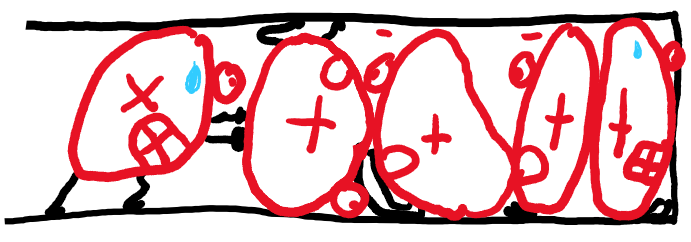
\includegraphics[width=0.8\textwidth]{Images/charges coincées.png}
\par\captionof{figure}{Des charges coincées dans un fil électrique}}

\only<3>{
Il faut \textbf{fermer} ou \textbf{court-circuiter}\par
\begin{circuitikz}
    \draw
    (0,0) to [V<=$U$] (0,4)
    to (3,4)
    to (3,0)
    to (0,0);
\end{circuitikz}}

\end{frame}

\begin{frame}{Les circuits sont des modèles}

\only<2>{

\includegraphics[width=0.8\textwidth, height=0.3\textwidth]{Images/Bleu.jpg}
\par\captionof{figure}{Dessin d'une partie finie de notre réservoir infini}}
\end{frame}

\begin{frame}
\title{La résistance à la rescousse, et découverte de la loi d'Ohm}
\titlepage
\end{frame}

\begin{frame}{La résistance}

\only<1>{
\begin{circuitikz}
    \draw
    (0,0) to [V<=$U$] (0,4)
    to (3,4)
    to [R=$R$, i=$I$] (3,0)
    to (0,0);
\end{circuitikz}}

\only<2,3>{
\begin{tcolorbox}
\centering \Large $\displaystyle I = \frac{U}{R}$
\end{tcolorbox}
\uncover<3>{\par $U=RI$}}

\only<4>{
Unité : ampère par volt [$\si{\ampere\per\volt}$] ou ohm [$\si{\ohm}$]
}
    
\end{frame}

\begin{frame}{Analogie hydraulique de la résistance}

\only<2>{
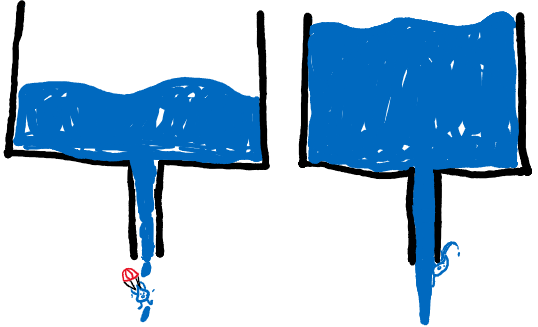
\includegraphics[height=0.55\textwidth]{Images/Résistance eau.png}
\par\captionof{figure}{Deux bacs d'eau avec un niveau différent}}

\only<3>{
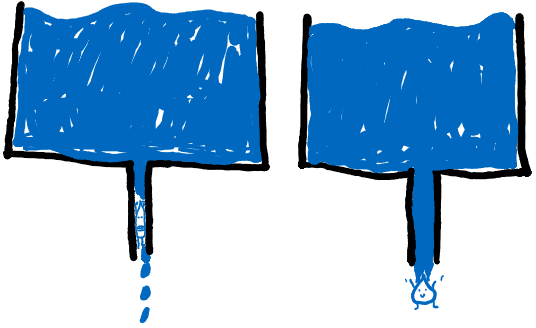
\includegraphics[height=0.55\textwidth]{Images/Résistance eau - bis.png}
\par\captionof{figure}{Deux bacs d'eau avec un tuyau différent}}

\end{frame}

\begin{frame}{Précision sur la tension}

\only<2-4>{Une tension\only<2>{ est une \emph{différence} de potentiel}\only<3,4>{ se mesure \emph{entre} deux points}
\uncover<4>{\par
\begin{circuitikz}
    \draw (0,0)
    to [V] (0,4)
    to (3,4)
    to [R, v^=$U$] (3,0)
    to (0,0);
\end{circuitikz}}}

\only<5>{
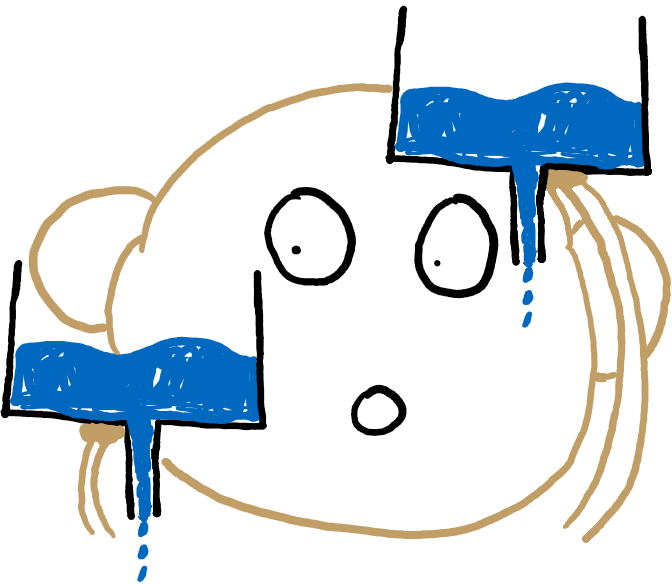
\includegraphics[height=0.5\textwidth]{Images/Même potentiel.png}
\captionof{figure}{Petit singe observant deux débits exactement égaux}}
    
\end{frame}

\begin{frame}{Résistance de l'air}
\only<2>{
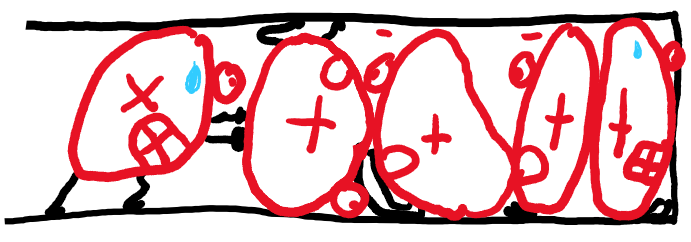
\includegraphics[width=0.8\textwidth]{Images/charges coincées.png}
\par\captionof{figure}{Des charges coincées dans un fil électrique}}
\end{frame}

\begin{frame}{Sens conventionnel du courant}
\end{frame}

\begin{frame}{Différentes conventions}
\only<2>{Voir dans le polycopié}
\end{frame}

\begin{frame}{La puissance}
\only<2>{Énergie par unité de temps : joule par seconde [$\si{\joule\per\second}$] ou watt [$\si{\watt}$]}
\end{frame}

\begin{frame}{Puissance mécanique}
\only<2,3>{
\begin{tabular}{m{0.5\textwidth}m{0.4\textwidth}}
\centering
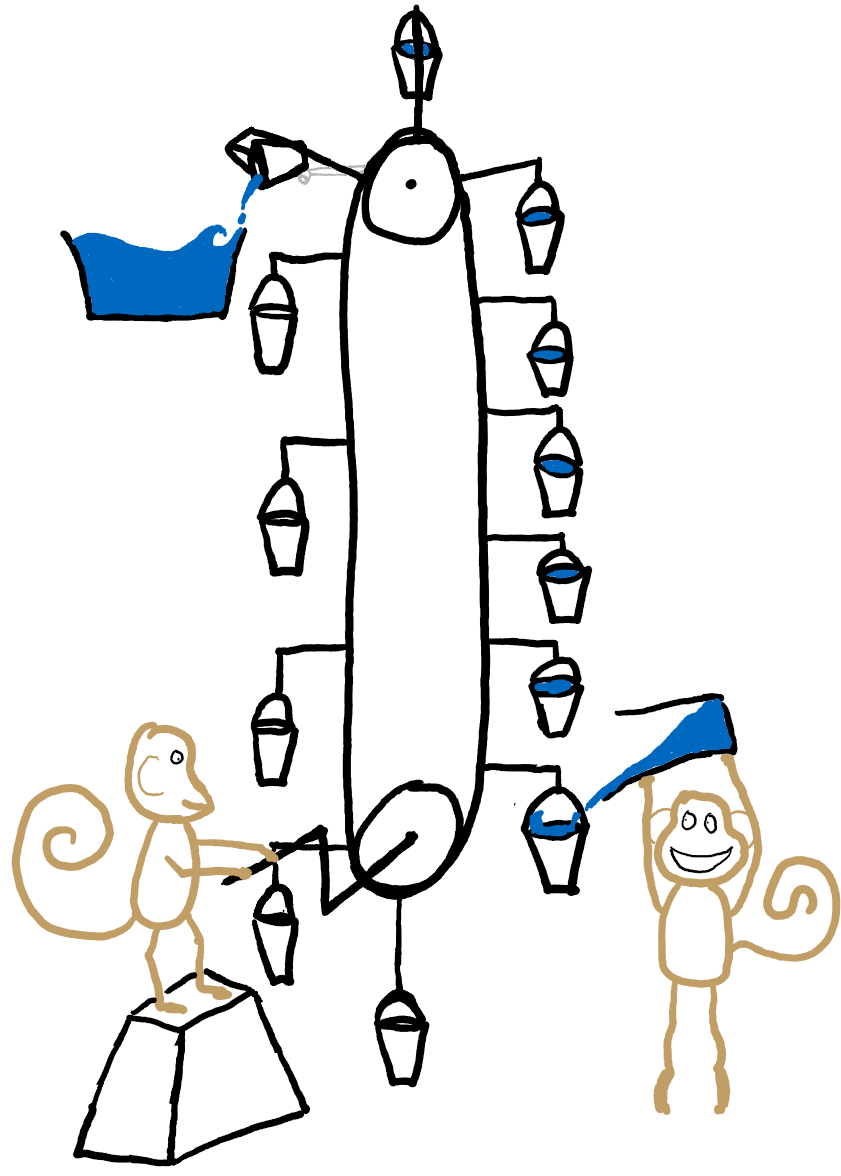
\includegraphics[height=0.6\textwidth]{Images/Singes pompent eau.png}
&
\centering
\uncover<3>{Puissance : $P=EF$}
\end{tabular}}
\end{frame}

\begin{frame}{Puissance électrique}
\only<2,3>{\begin{tabular}{m{0.5\textwidth}m{0.4\textwidth}}
\centering
\begin{circuitikz}
\draw (0,4) to [V=$U$] (0,0);
\draw (0,4) to [short, i=$I$] (3,4)
to [R=$R$] (3,0)
to (0,0);
\end{circuitikz}
&
\centering
\uncover<3>{
\begin{tcolorbox}[title=Puissance]
\centering $P=UI$
\end{tcolorbox}}
\end{tabular}}
\end{frame}

\begin{frame}
\title{Quiz !}
\titlepage
\par responseware.eu, ID : s4s1
\end{frame}

\begin{frame}{Quiz : réponses}
\end{frame}

\begin{frame}
\title{Circuits plus complexes}
\titlepage    
\end{frame}

\begin{frame}{Source de courant}
\only<2,3>{
\begin{tabular}{*2{m{0.45\textwidth}}}
\centering
\begin{circuitikz}
    \draw (0,4) [V_=$U$] to (0,0);
    \draw (0,4) to (3,4)
    to [R, l_=$R$, i=$I$] (3,0)
    to (0,0);
\end{circuitikz}
\uncover<3>{\par \vspace{3pt} $\displaystyle I=\frac{U}{R}$}&
\centering
\begin{circuitikz}
    \draw (0,0) [I=$I$] to (0,4);
    \draw (0,4) to (3,4)
    to [R, l_=$R$, v^=$U$] (3,0)
    to (0,0);
\end{circuitikz}
\uncover<3>{\par $U=RI$}
\end{tabular}}
\end{frame}

\begin{frame}{Dualité courant-tension}
\only<2>{
\begin{tabular}{*3{m{0.24\textwidth}}}
\centering
$\displaystyle I=\frac{U}{R}$ & \centering $\equiv$ & \centering $U=RI$
\end{tabular}}
\end{frame}

\begin{frame}{Chute de tension}
\only<2>{
\begin{circuitikz}
\draw (0,4) [V_=$U$] to (0,0);
\draw (0,4) to (3,4)
to [R, l_=$R$, i=$I$] (3,0)
to (0,0);
\end{circuitikz}}
\end{frame}

\begin{frame}
\title{Branchement en série et en parallèle}
\titlepage
\end{frame}

\begin{frame}{Branchement en parallèle}

\only<1>{
\begin{circuitikz}
\draw
  (-0.5,0) to [V_<=$U$] (-0.5,4) 
  to [short, -*, i=$\underline{I}$] (2,4)
  to [R, l_=$R_1$, -*, i>_=$I_1$, v^=$U_1$] (2,0) 
  to (-0.5,0)
  (2,4) to [short, i=$I_2$] (4,4)
  to [R, l_=$R_2$, v^=$U_2$] (4,0)
  to (2,0);
\end{circuitikz}}

\only<2>{
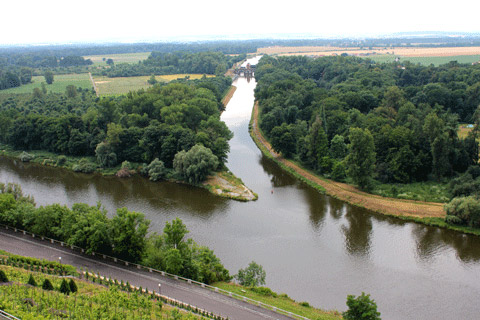
\includegraphics[height=0.4\textwidth]{Images/riverBifurcation.jpg}
\captionof{figure}{Cours d'eau se séparant en deux}}
    
\end{frame}

\begin{frame}{Branchement en série}

\only<1>{
\begin{circuitikz}
\draw
  (0,0) to [V_<=$U$] (0,4)
  to [short, i=$I$] (3,4);
\ctikzset{current/distance = 0.8}
\draw
  (3,4) to [R, l_=$R_1$, i_=$I$, v^=$U_1$] (3,2)
  to [R, l_=$R_2$, v^=$U_2$] (3,0)
  to [short ] (0,0);
\end{circuitikz}}

\only<2>{
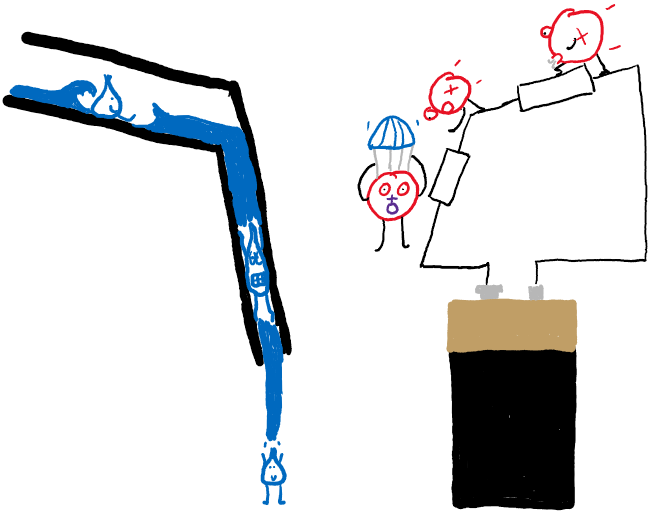
\includegraphics[height=0.55\textwidth]{Images/Diviseur tension.png}
\captionof{figure}{Chute de hauteur, et chute de tension}}
    
\end{frame}

\begin{frame}
\title{N\oe{}uds, branches et mailles}
\titlepage
\end{frame}

\begin{frame}{N\oe{}uds}

\only<2>{
\begin{tabular}{*2{m{0.45\textwidth}}}
\centering
\begin{circuitikz}
\draw
  (0,0) to [R, l_=$R$] (2,0)
  to [R, *- , l_=$R$] (4,2)
  (2,0) to [R, l_=$R$] (4,-2);
\end{circuitikz}
&
\centering
\begin{circuitikz}
\draw
  (0,0) to [R, l_=$R$] (0,4) 
  to [short] (1,4)
  to [short, *-] (2,4)
  to [short, *-] (3,4)
  (1,0)  to [R, l_=$R$] (1,4) 
  (2,0)to [R, l_=$R$] (2,4)
  (3, 0) to [R, l_=$R$,] (3,4);
\end{circuitikz}
\end{tabular}}

\only<3>{
Exemple\par
\begin{circuitikz}
\draw
  (-0.5,0) to [V_<=$U$] (-0.5,4) 
  to [short] (2,4)
  to [R, l_=$R_3$] (2,0) 
  to [short, *- ] (-0.5,0)
  (2,4) to [short, *-] (4,4)
  to [R, l_=$R_1$] (4,2) 
  to [R, l_=$R_2$] (4,0)
  to [short] (2,0);
\end{circuitikz}}
\end{frame}

\begin{frame}{Branches}

\only<2>{
\begin{circuitikz}
\draw
  (-0.25,0) to [short, *-] (0,0)
  to [R] (2, 0)
  to [R] (4, 0)
  to [L] (6, 0)
  to [R] (8, 0)
  to [C] (9, 0)
  to [short, -*] (9.5, 0);
\end{circuitikz}
\par Une branche constituée de plusieurs dipôles
}

\only<3>{
Exemple\par
\begin{circuitikz}
\draw
  (-0.5,0) to [V_<=$U$] (-0.5,4) 
  to [short] (2,4)
  to [R, l_=$R_3$] (2,0) 
  to [short, *- ] (-0.5,0)
  (2,4) to [short, *-] (4,4)
  to [R, l_=$R_1$] (4,2) 
  to [R, l_=$R_2$] (4,0)
  to [short] (2,0);
\end{circuitikz}}

\only<4>{
\begin{tabular}{m{0.28\textwidth}cm{0.2\textwidth}cm{0.28\textwidth}}
\centering
\begin{circuitikz}
\draw
    (0,0) to [V_<=$U$] (0,4)
    to [short, -*] (1.5,4)
    (0,0) to [short, -*] (1.5,0);
\end{circuitikz}
&$+$&
\centering
\begin{circuitikz}
\draw (0,0) to [R=$R_3$, *-*] (0,4);
\end{circuitikz}
&$+$&
\centering
\begin{circuitikz}
\draw
    (0,0) to [short, *-] (1.5,0)
    to [R=$R_2$] (1.5,2)
    to [R=$R_1$] (1.5,4)
    to [short, -*] (0,4);
\end{circuitikz}
\end{tabular}}
\end{frame}

\begin{frame}{Mailles}

\only<2>{
\begin{circuitikz}
\draw
  (0,0) to [R, l_=$R_3$] (0,4) 
  to [short] (2.5,4)
  to [R, l_=$R_1$] (2.5,2) 
  to [R, l_=$R_2$] (2.5,0)
  to [short] (0,0);
\end{circuitikz}
\par Maille composée de 3 résistances}

\only<3>{
Exemple\par
\begin{circuitikz}
\draw
  (-0.5,0) to [V_<=$U$] (-0.5,4) 
  to [short] (2,4)
  to [R, l_=$R_3$] (2,0) 
  to [short, *- ] (-0.5,0)
  (2,4) to [short, *-] (4,4)
  to [R, l_=$R_1$] (4,2) 
  to [R, l_=$R_2$] (4,0)
  to [short] (2,0);
\end{circuitikz}}

\only<4>{
\begin{tabular}{m{0.26\textwidth}cm{0.28\textwidth}cm{0.26\textwidth}}
\centering
\begin{circuitikz}
\draw
  (-0.5,0) to [V_<=$U$] (-0.5,4) 
  to [short] (2,4)
  to [R, l_=$R_3$] (2,0) 
  to [short] (-0.5,0);
\end{circuitikz}
& $+$ &
\centering
\begin{circuitikz}
\draw
  (-0.5,0) to [V_<=$U$] (-0.5,4) 
  to [short] (2,4)
  to [R, l_=$R_1$] (2,2) 
  to [R, l_=$R_2$] (2,0)
  to [short] (-0.5,0);
\end{circuitikz}
& $+$ &
\centering
\begin{circuitikz}
\draw
  (0,0) to [R, l_=$R_3$] (0,4) 
  to [short] (2,4)
  to [R, l_=$R_1$] (2,2) 
  to [R, l_=$R_2$] (2,0)
  to [short] (0,0);
\end{circuitikz}
\end{tabular}}
\end{frame}

\begin{frame}{Définitions plus précises}
\only<-3>{
\begin{tcolorbox}[title=Parallèle et série]
\begin{itemize}
    \item<2-> Deux dipôles en série sont montés sur la même branche.
    \item<3> Deux dipôles en parallèle sont montés sur deux branches reliées aux mêmes n\oe{}uds.
\end{itemize}
\end{tcolorbox}}

\only<4-6>{
\begin{tcolorbox}[title=Intuition]
\begin{itemize}
    \item<5-> Deux dipôles en série sont parcourus par le même courant. De plus, ils se partagent la tension totale.
    \item<6> Deux dipôles en parallèles ont la même tension à leurs bornes. De plus, ils se partagent le courant total.
\end{itemize}
\end{tcolorbox}}
\end{frame}

\begin{frame}
\title{Lois de Kirchhoff}
\titlepage
\end{frame}

\begin{frame}{Lois de n\oe{}uds}
\begin{tabular}{ccc}
\begin{circuitikz}
\draw
  (0,0) to [short, i_=$i_0$] (1.5,0)
  to [short, *- , i^=$i_1$] (3,1.5)
  (1.5,0) to [short, i^=$i_2$] (3,-1.5);
\end{circuitikz}
&
\begin{circuitikz}
\draw
  (-1.5,1.5) to [short, i^=$i_3$] (0,0)
  to [short, *- , i^=$i_5$] (1.5,0)
  (-1.5,-1.5) to [short, i^=$i_4$] (0,0);
\end{circuitikz}
&
\begin{circuitikz}
\draw
  (-1.5,1.5) to [short, i^=$i_6$] (0,0)
  to [short, i^=$i_8$] (1.5,1.5)
  (-1.5,-1.5) to [short, i^=$i_7$] (0,0)
  to [short, *- , i^=$i_9$] (1.5,-1.5);
\end{circuitikz}
\end{tabular}
\end{frame}

\begin{frame}{Loi des mailles, première variante}
\only<2>{
Exemple\par
\begin{circuitikz}
\draw
  (-0.5,0) to [V_<=$U$] (-0.5,4) 
  to [short] (2,4)
  to [R, l_=$R_3$] (2,0) 
  to [short, *- ] (-0.5,0)
  (2,4) to [short, *-] (4,4)
  to [R, l_=$R_1$] (4,2) 
  to [R, l_=$R_2$] (4,0)
  to [short] (2,0);
\end{circuitikz}}

\only<3>{
\begin{tabular}{m{0.26\textwidth}cm{0.28\textwidth}cm{0.26\textwidth}}
\centering
\begin{circuitikz}
\draw
  (-0.5,0) to [V_<=$U$] (-0.5,4) 
  to [short] (2,4)
  to [R, l_=$R_3$] (2,0) 
  to [short] (-0.5,0);
\end{circuitikz}
& $+$ &
\centering
\begin{circuitikz}
\draw
  (-0.5,0) to [V_<=$U$] (-0.5,4) 
  to [short] (2,4)
  to [R, l_=$R_1$] (2,2) 
  to [R, l_=$R_2$] (2,0)
  to [short] (-0.5,0);
\end{circuitikz}
& $+$ &
\centering
\begin{circuitikz}
\draw
  (0,0) to [R, l_=$R_3$] (0,4) 
  to [short] (2,4)
  to [R, l_=$R_1$] (2,2) 
  to [R, l_=$R_2$] (2,0)
  to [short] (0,0);
\end{circuitikz}
\end{tabular}}
\end{frame}

\begin{frame}{Loi des mailles, deuxième variante}
\only<2>{
Exemple\par
\begin{circuitikz}
\draw
  (-0.5,0) to [V_<=$U$] (-0.5,4) 
  to [short] (2,4)
  to [R, l_=$R_3$] (2,0) 
  to [short, *- ] (-0.5,0)
  (2,4) to [short, *-] (4,4)
  to [R, l_=$R_1$] (4,2) 
  to [R, l_=$R_2$] (4,0)
  to [short] (2,0);
\end{circuitikz}}

\only<3>{
\begin{tabular}{m{0.28\textwidth}cm{0.20\textwidth}cm{0.28\textwidth}}
\centering
\begin{circuitikz}
\draw
    (0,0) to [V_<=$U$] (0,4)
    to [short, -*] (1.5,4)
    (0,0) to [short, -*] (1.5,0);
\end{circuitikz}
&$+$&
\centering
\begin{circuitikz}
\draw (0,0) to [R=$R_3$, *-*] (0,4);
\end{circuitikz}
&$+$&
\centering
\begin{circuitikz}
\draw
    (0,0) to [short, *-] (1.5,0)
    to [R=$R_2$] (1.5,2)
    to [R=$R_1$] (1.5,4)
    to [short, -*] (0,4);
\end{circuitikz}
\end{tabular}}
\end{frame}

\begin{frame}{Lois de Kirchhoff}
\begin{tcolorbox}[title=Pour résumer]
\begin{itemize}
    \small
    \item<2-> \textbf{La loi des n\oe{}uds} dit que la somme algébriques des courants entrants dans un n\oe{}ud est égale à celle des courants sortants.
    \item<3-> \textbf{La loi des mailles} dit que la somme algébriques des tensions aux bornes des dipôles d'une maille est nulle.
    \item<4> \textbf{Une formulation équivalente} de la loi des mailles dit que les deux sommes algébrique des tensions aux bornes des dipôles de deux branches connectées aux mêmes n\oe{}uds sont égales.
\end{itemize}
\end{tcolorbox}
\end{frame}

\begin{frame}{Diviseur de tension}
\only<1>{
\begin{circuitikz}
\draw
  (0,0) to [V_<=$U$] (0,4)
  to [short, i=$I$] (3,4);
\ctikzset{current/distance = 0.8}
\draw
  (3,4) to [R, l_=$R_1$, i_=$I$, v^=$U_1$] (3,2)
  to [R, l_=$R_2$, v^=$U_2$] (3,0)
  to [short ] (0,0);
\end{circuitikz}}

\only<2>{
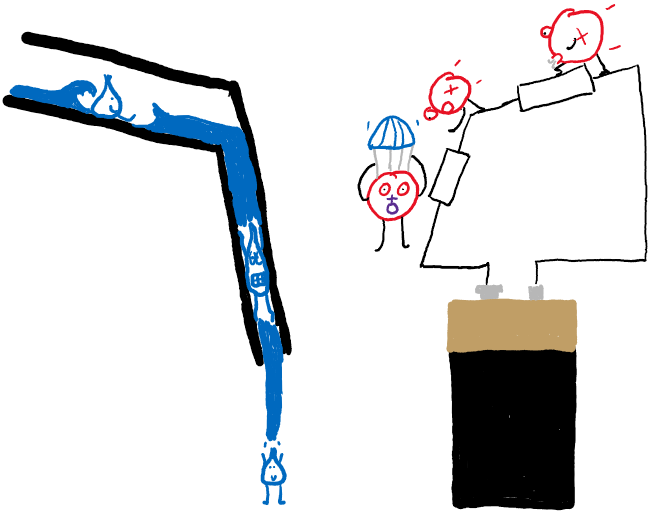
\includegraphics[height=0.55\textwidth]{Images/Diviseur tension.png}
\captionof{figure}{Chute de hauteur, et chute de tension}}
\end{frame}

\begin{frame}{Exemple : diviseur de courant}
\begin{circuitikz}
\draw
    (0,0) to [isource=$I$] ++(0,4)
    to ++(6,0)
    to [R=$R_2$, i>^=$I_2$, v=$U_2$] ++(0,-4)
    to (0,0)
    (3,4) to [R=$R_1$, *-*, i>^=$I_1$, v=$U_1$] ++(0,-4);
\end{circuitikz}
\vspace{2.2cm}
\end{frame}

\begin{frame}{Simplification de circuits}

\only<2,3>{
\begin{tabular}{m{0.4\textwidth}cm{0.3\textwidth}}
\raggedleft
\begin{circuitikz}
\draw
  (0,0) to [R, l^=$R_1$] (3,0) 
  (3,0) to (3,1) 
  (3,1) to [short, *-] (3,1.5) 
  (3,1.5) to [R, l_=$R_2$] (0,1.5)
  (3,1) to (4, 1) 
  (4,1) to (4,-1.5) 
  (4,-1.5) to [R, l_=$R_3$](0,-1.5) 
  ;
\end{circuitikz}
&
\uncover<3>{\centering
$\equiv$
&
\raggedright
\begin{circuitikz}
\draw
  (4,1) to [R, l^=$R_1$] (7,1) 
  (7,1) to (7,2) 
  (7,2) to [short, *-] (7,3) 
  (7,3) to [R, l_=$R_3$] (4,3)
  (4,2) to [R, l^=$R_2$] (7,2);
\end{circuitikz}}
\end{tabular}}

\only<4,5>{
\begin{tabular}{m{0.37\textwidth}m{0.43\textwidth}}
\raggedleft
\begin{circuitikz}[scale=0.8, transform shape]
\draw
 (1,0) to [european voltage source, *-] (1,2)
 (1,2) to [R, l_=$R_0$](1,4)
 (1,4) to [short, *-](0,4) 
 (0,4) to [R, l_=$R_1$](0,0) 
 (0,0) to (1,0) 
 (1,4) to [short, *-](3,4)
 (3,4) to [R, l_=$R_2$](3,1.7)
 (3,1.7) to [R, l^=$R_3$](2,0)
 (3,3.8) to[short, *-] (2, 3.8)
 (2,3.8) to [R, l_=$R_4$](2, 0)
 (2,0) to [short, *-](1, 0)
 (3,3.6) to [short, *-](4, 3.6)
 (4,3.6) to [R, l_=$R_5$](4, 0)
 (4, 0) to [short, *-](2, 0)
 ;
\end{circuitikz}
&
\uncover<5>{
\raggedright
\begin{circuitikz}[scale=0.8, transform shape]
\draw
(0,0) to [european voltage source] (0,4)
 (0,4) to [R, l_=$R_0$] (2,4)
 (2,4) to (5,4)
 (2,4) to [R, l_=$R_1$, *-] (2,0)
 (4,4) to [R, l_=$R_4$, *-] (4,0)
 (3,4) to [R, l_=$R_2$, *-] (3,2)
 (3,2) to [R, l_=$R_3$] (3,0)
 (5,4) to [R, l^=$R_5$] (5,0)
 (5,0) to [short](4,0)
 (4,0) to [short, *-](3,0)
 (3,0) to [short, *-](2,0)
 (2,0) to [short, *-](0,0)
  ;
\end{circuitikz}}
\end{tabular}}
\end{frame}

\begin{frame}
\title{Sources réelles}
\titlepage
\end{frame}

\begin{frame}{Source de tension réelle}
\only<2>{Problème :\par
\begin{circuitikz}
\draw
    (0,3)
    to [V=$\SI{5}{\volt}$] (0,0)
    (0,3) to (2.5,3) node[anchor=west]{$a$}
    to [short, o-o] (2.5,0) node[anchor=west]{$b$}
    to (0,0)
 ;
\end{circuitikz}}

\only<3>{Solution :\par
\begin{circuitikz}
\draw (0,3) to [V=$\SI{5}{\volt}$] (0,0)
(0,3) to [R, l_=$R_i$, -o] (2.5,3) node[anchor=west]{$a$}
(0,0) to [short, -o] (2.5,0) node[anchor=west]{$b$};
\draw[dashed] (-0.7,-0.3) rectangle (2.1,3.5);
\end{circuitikz}}

\only<4->{
\begin{tabular}{*2{m{0.4\textwidth}}}
\centering
\begin{circuitikz}
\draw (0,3) to [V=$\SI{5}{\volt}$] (0,0)
(0,3) to [R, l_=$R_i$, -o] (2.5,3) node[anchor=west]{$a$}
to [short, -o] (2.5,0) node[anchor=west]{$b$}
to (0,0);
\draw[dashed] (-0.7,-0.3) rectangle (2.1,3.5);
\end{circuitikz}
&
\centering
\uncover<5>{
\begin{circuitikz}
\draw (0,3) to [V=$\SI{5}{\volt}$] (0,0)
(0,3) to [R, l_=$R_i$, -o] (2.5,3) node[anchor=west]{$a$}
to [R=$R$, -o] (2.5,0) node[anchor=west]{$b$}
to (0,0);
\draw[dashed] (-0.7,-0.3) rectangle (2.1,3.5);
\end{circuitikz}}
\end{tabular}}
\end{frame}

\begin{frame}{Source de courant réel}
\only<2>{
Problème :\par
\begin{circuitikz}
\draw
(0,0) to [I=$\SI{1}{\ampere}$] (0,3)
to [short, -o] (2,3) node[anchor=west]{$a$}
(2,0) node[anchor=west]{$b$}
to [short, o-] (0,0);
\end{circuitikz}}

\only<3->{
Solution :\par

\begin{tabular}{*3{m{0.3\textwidth}}}
\centering
\begin{circuitikz}[scale=0.8, transform shape]
\draw (0,0)
to [I_=$\SI{1}{\ampere}$] (0,3)
to [short, -*] (1.5,3)
to [R, l^=$R_i$, -*] (1.5,0)
to (0,0)
(1.5,3) to [short, -o] (3,3) node[anchor=west]{$a$}
(1.5,0) to [short, -o] (3,0) node[anchor=west]{$b$};
\draw[dashed] (-0.7,-0.3) rectangle (2.5,3.3);
\end{circuitikz}
&
\uncover<4->{
\centering
\begin{circuitikz}[scale=0.8, transform shape]
\draw (0,0)
to [I_=$\SI{1}{\ampere}$] (0,3)
to [short, -*] (1.5,3)
to [R, l^=$R_i$, -*] (1.5,0)
to (0,0)
(1.5,3)
to [short, -o] (3,3) node[anchor=west]{$a$}
to [short, -o] (3,0) node[anchor=west]{$b$}
to (1.5,0);
\draw[dashed] (-0.7,-0.3) rectangle (2.5,3.3);
\end{circuitikz}}
&
\uncover<5>{
\centering
\begin{circuitikz}[scale=0.8, transform shape]
\draw (0,0)
to [I_=$\SI{1}{\ampere}$] (0,3)
to [short, -*] (1.5,3)
to [R, l^=$R_i$, -*] (1.5,0)
to (0,0)
(1.5,3)
to [short, -o] (3,3) node[anchor=west]{$a$}
to [R=$R$, -o] (3,0) node[anchor=west]{$b$}
to (1.5,0);
\draw[dashed] (-0.7,-0.3) rectangle (2.5,3.3);
\end{circuitikz}}
\end{tabular}}
\end{frame}

\begin{frame}
\title{Quiz !}
\titlepage
\par responseware.eu, ID : s4s1
\end{frame}

\begin{frame}{Quiz : réponses}
\end{frame}

\begin{frame}
\title{Éléments réactifs}
\titlepage
\end{frame}

\begin{frame}{Le condensateur}

\only<2>{
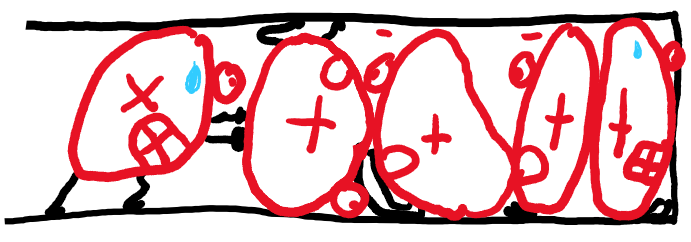
\includegraphics[width=0.8\textwidth]{Images/charges coincées.png}
\par\captionof{figure}{Des charges coincées dans un fil électrique}}

\only<3>{
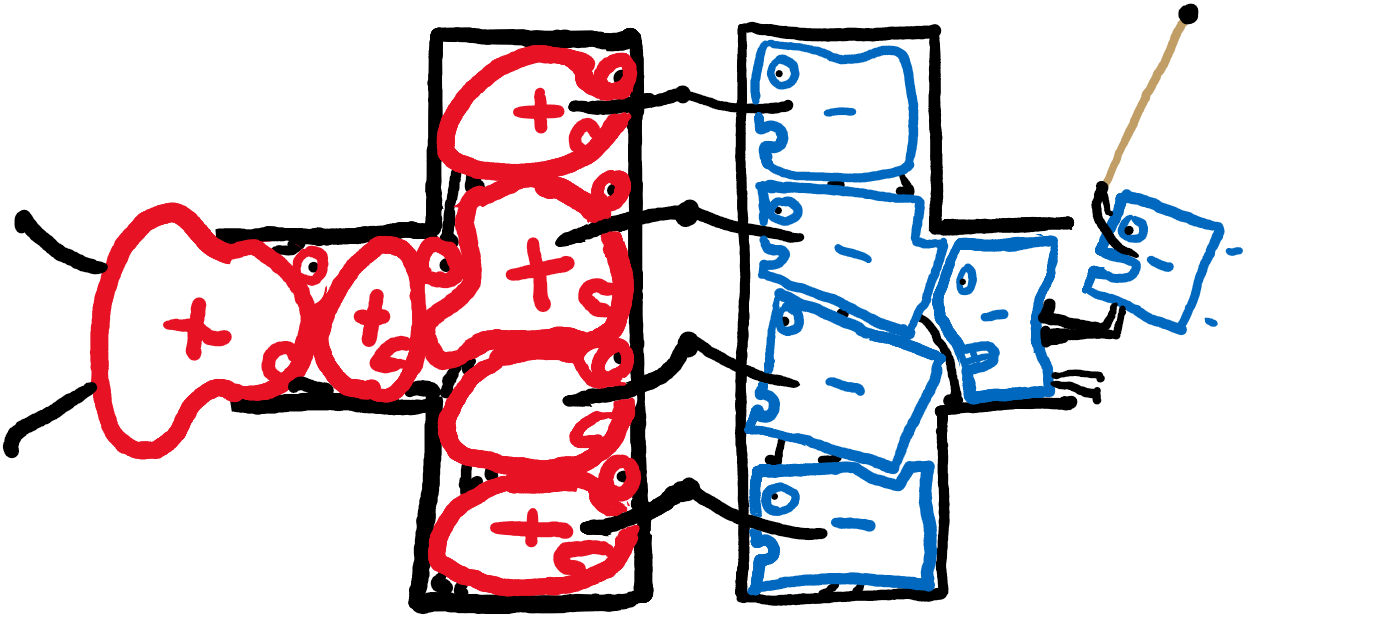
\includegraphics[width=0.8\textwidth]{Images/Condensateur.png}
\par\captionof{figure}{Deux plaques forment un condensateur}}

\only<4,5>{
\begin{circuitikz}
\draw (0,0) to [C=$C$, v_=$u$] (4,0);
\end{circuitikz}
\uncover<5>{
\begin{tcolorbox}
\[ Q = Cu \]
\end{tcolorbox}}}

\only<6>{
Unité : coulomb par volt [$\si{\coulomb\per\volt}$] ou farad [$\si{\farad}$]}
\end{frame}

\begin{frame}{Analogie hydraulique}
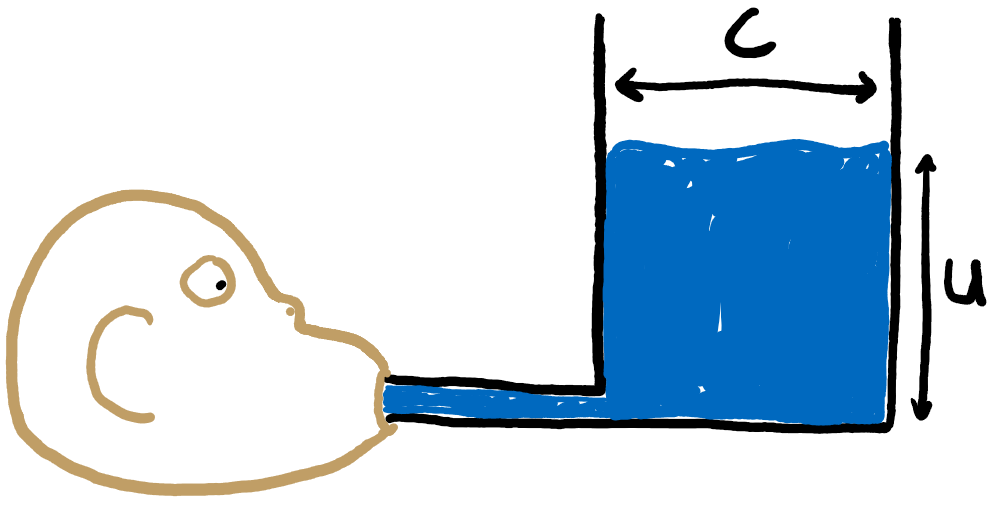
\includegraphics[height=0.4\textwidth]{Images/Condensateur CU.png}
\captionof{figure}{Le singe doit souffler pour ne pas se noyer}
\end{frame}

\begin{frame}{L'équation du condensateur}
\only<2-4>{
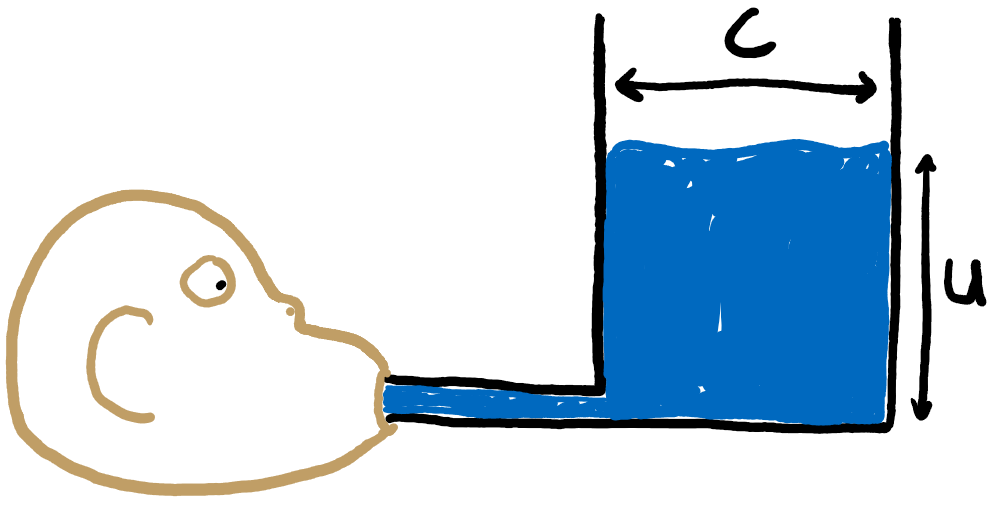
\includegraphics[height=0.2\textwidth]{Images/Condensateur CU.png}
\begin{align*}
    Q &= Cu \\
    \uncover<3-4>{\frac{\mathrm{d}Q}{\mathrm{d}t} &= C\frac{\mathrm{d}u}{\mathrm{d}t}} \\
    \uncover<4>{i &= C\frac{\mathrm{d}u}{\mathrm{d}t}}
\end{align*}}

\only<5>{
\begin{circuitikz}
\draw (0,0) to [C=$C$, i=$i$, v=$u$] (4,0);
\end{circuitikz}
\[i = C\frac{\mathrm{d}u}{\mathrm{d}t}\]}
\end{frame}

\begin{frame}{Remarque}

\uncover<2->{
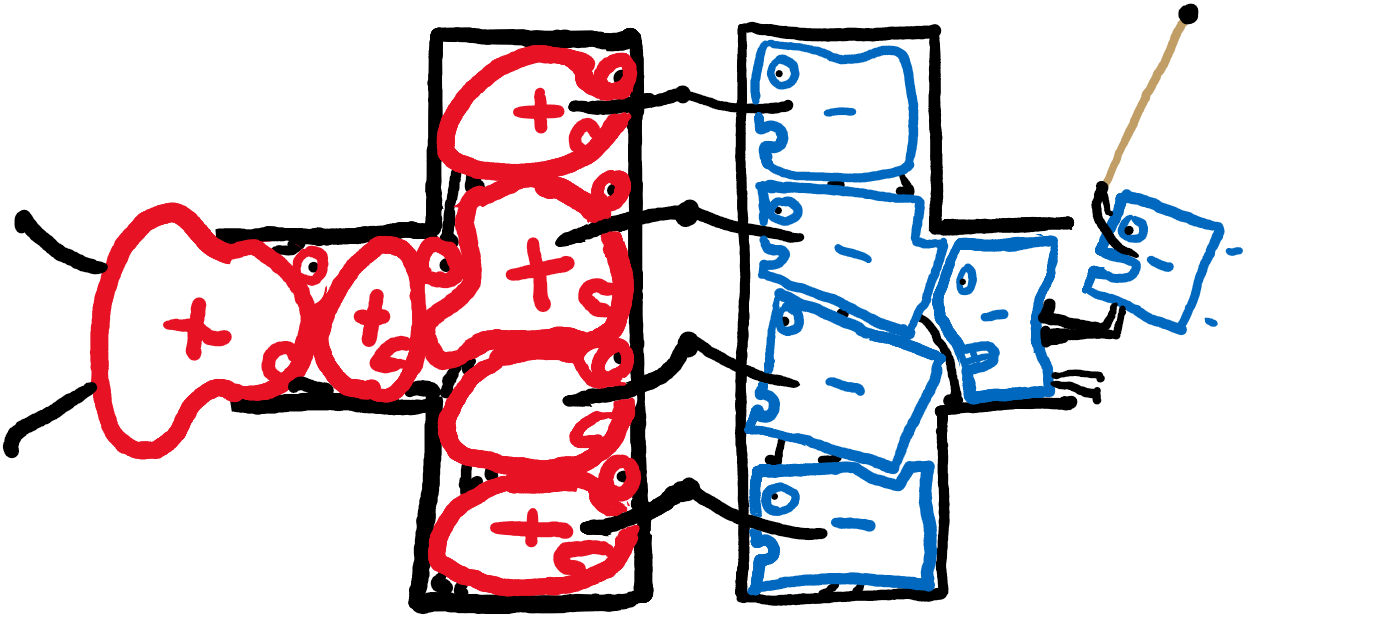
\includegraphics[height=0.3\textwidth]{Images/Condensateur.png}}
\par
\uncover<3->{
\begin{circuitikz}
\draw (0,0)
to [short, i=$i_1$] (1.8,0)
to [C] (2.2,0)
to [short, i=$i_2$] (4,0);
\end{circuitikz}}
\uncover<4>{\par
$i_1 = i_2$}
\end{frame}

\begin{frame}{La bobine}
\only<2>{
\begin{circuitikz}
\draw (0,0) to [L=$L$] (4,0);
\end{circuitikz}}
\end{frame}

\begin{frame}{Analogie hydraulique}
\only<2>{Les choses commencent à se casser.}

\only<3>{
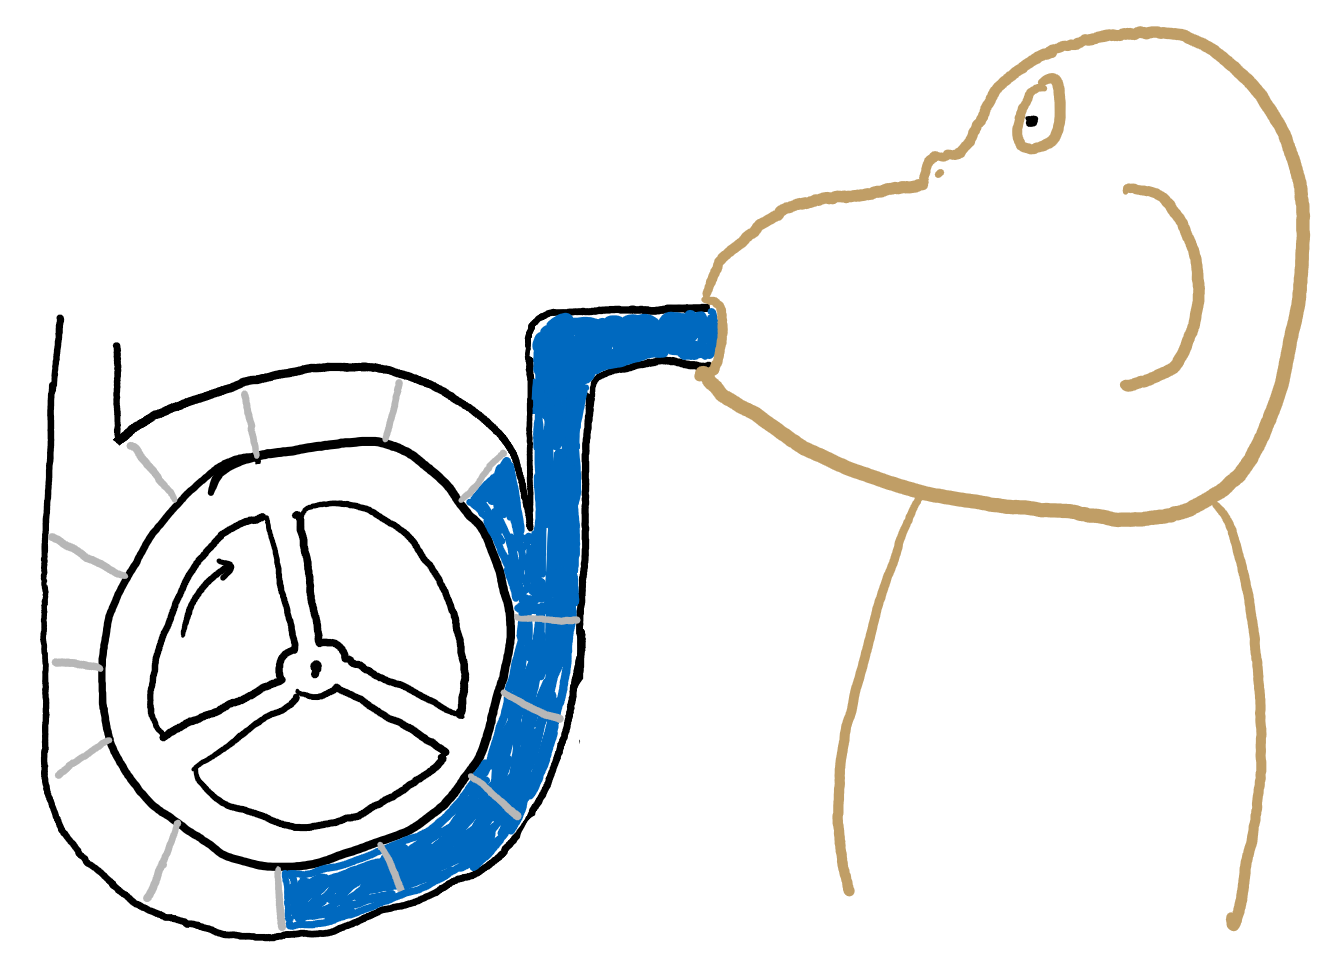
\includegraphics[height=0.5\textwidth]{Images/Bobine inertie.png}
\captionof{figure}{Volant d'inertie analogue à une bobine}}
\end{frame}

\begin{frame}{Équation de la bobine}
\only<2-4>{
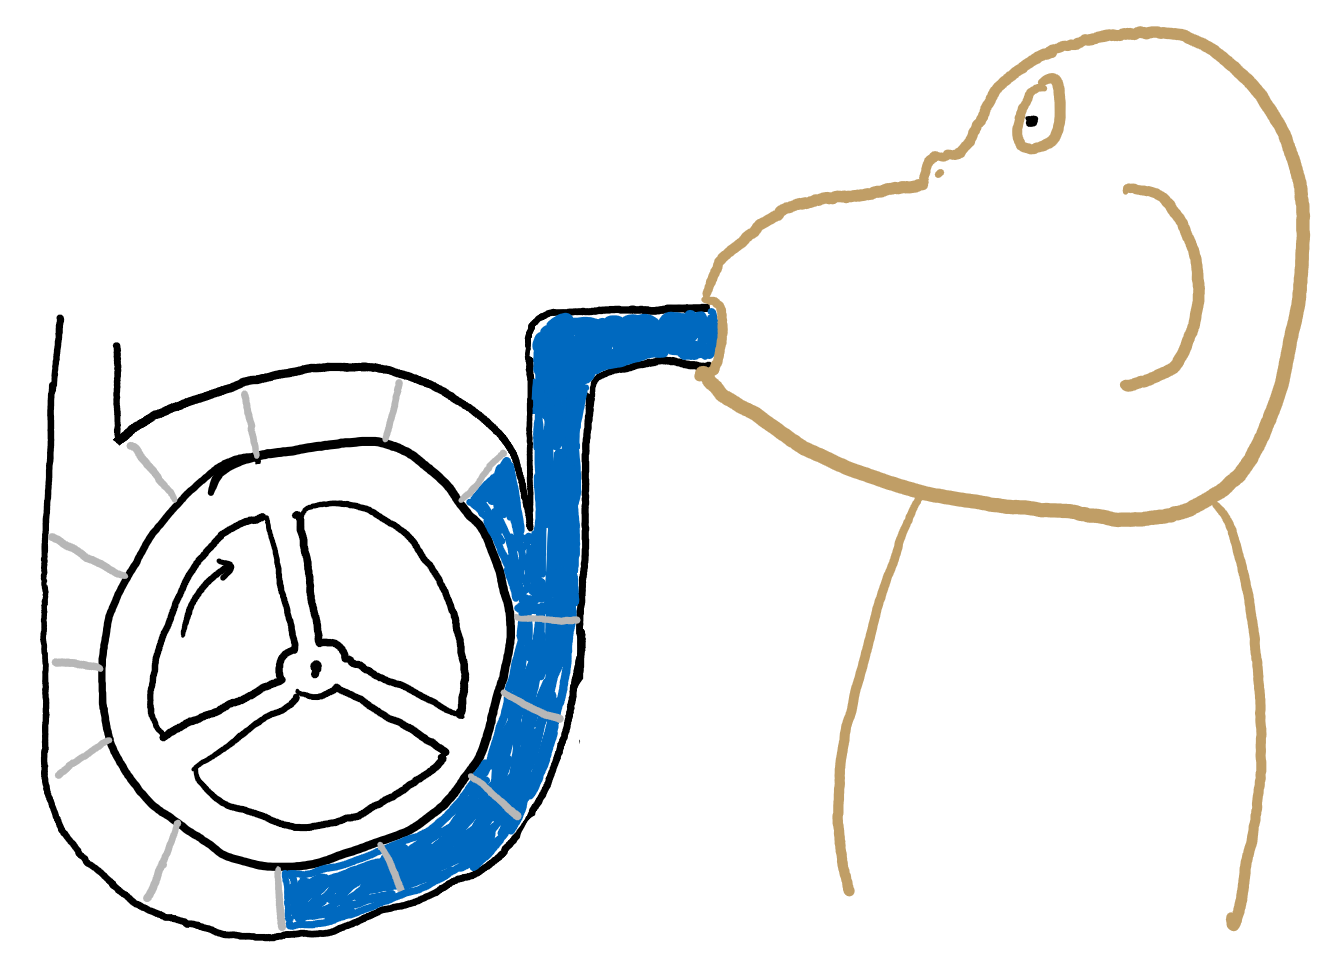
\includegraphics[height=0.25\textwidth]{Images/Bobine inertie.png}
\begin{align*}
    \uncover<2-4>{F &= ma}\\
    \uncover<3-4>{F &= m\frac{\mathrm{d}D}{\mathrm{d}t}}\\
    \uncover<4>{u &= L\frac{\mathrm{d}i}{\mathrm{d}t}}
\end{align*}}

\only<5>{
\begin{circuitikz}
\draw (0,0) to [L=$L$, i=$i$, v=$u$] (4,0);
\end{circuitikz}
\[u = L\frac{\mathrm{d}i}{\mathrm{d}t}\]}

\only<6>{
Unité : volt par (ampère par seconde) [$\si{\volt\per\ampere\second}$] ou henry [$\si{\henry}$]}

\end{frame}

\begin{frame}
\title{Résolution de systèmes simples}
\titlepage
\end{frame}

\begin{frame}{Circuit RC}

\only<2>{
Charge\par
\begin{circuitikz}
\draw
  (0,0) to [V<=$U$] (0,4) 
  to [R, l_=$R$, v^=$u_R$] (3,4)
  to [C, i>^= $i$, l_=$C$, v^=$u_C$] (3,0) 
  to (0,0);
\end{circuitikz}\hfill}

\only<3>{
Décharge\par
\begin{circuitikz}
\draw (0,0) to [C, l_=$C$, v^<=$u$] (0,4)
to [short, i=$i$] (3,4)
to [R=$R$] (3,0)
to (0,0);
\end{circuitikz}\hfill}

\end{frame}

\begin{frame}{Circuit RL}

\only<2>{
\og Charge \fg\par
\begin{circuitikz}
\draw
  (0,0) to [V<=$U$] (0,4) 
  to [R, l_=$R$, v^=$u_R$] (3,4)
  to [L, i>_= $i$, l_=$L$, v^=$u_L$] (3,0) 
  to (0,0);
\end{circuitikz}\hfill}

\only<3>{
\og Décharge \fg\par
\begin{circuitikz}
\draw (0,0) to [L, l_=$L$, v^<=$u$] (0,4)
to [short, i=$i$] (3,4)
to [R=$R$] (3,0)
to (0,0);
\end{circuitikz}\hfill}
\end{frame}

\begin{frame}
\title{Intuitions supplémentaires}
\titlepage
\end{frame}

\begin{frame}{Le régime permanent}

\only<2,3>{
\begin{tabular}{m{0.4\textwidth}cm{0.4\textwidth}}
\centering
\begin{circuitikz}[scale=0.8, transform shape]
\draw
  (0,0) to [V<=$U$] (0,4) 
  to [R, l_=$R$] (3,4)
  to [C, i>^= $i$, l_=$C$, v^=$u_C$] (3,0) 
  to (0,0);
\end{circuitikz}
& \uncover<3>{\centering $\equiv$ \normalsize &
\centering
\begin{circuitikz}[scale=0.8, transform shape]
\draw
  (0,0) to [V<=$U$] (0,4) 
  to [R, l_=$R$, i_>=$i$] (3,4)
  to [open, o-o, v^=$u_C$] (3,0) 
  to (0,0);
\end{circuitikz}}
\end{tabular}}

\only<4->{
\begin{tabular}{m{0.4\textwidth}cm{0.4\textwidth}}
\begin{circuitikz}[scale=0.8, transform shape]
\draw
  (0,0) to [V<=$U$] (0,4) 
  to [R, l_=$R$] (3,4)
  to [L, i>^= $i$, l_=$L$, v^=$u_L$] (3,0) 
  to (0,0);
\end{circuitikz}
& \uncover<5>{\centering $\equiv$ \normalsize &
\centering
\begin{circuitikz}[scale=0.8, transform shape]
\draw
  (0,0) to [V<=$U$] (0,4) 
  to [R, l_=$R$, i_>=$i$] (3,4)
  to [short, *-*, v^=$u_L$] (3,0) 
  to (0,0);
\end{circuitikz}}
\end{tabular}}
\end{frame}

\begin{frame}{Les cas interdits}
\only<2,3>{
\begin{tabular}{*2{c}}
\begin{circuitikz}
\draw (0,0)
    to [C, v^<=$u_C$] (0,4)
    to (2,4)
    to [short] (2,0)
    to (0,0);
\end{circuitikz}
&\uncover<3>{
\begin{circuitikz}
\draw (0,0)
    to [C, v^<=$u_C$] (0,4)
    to (2,4)
    to [V=$U$] (2,0)
    to (0,0);
\end{circuitikz}}\\
$u_C \neq 0$ & \uncover<3>{$u_C \neq U$}
\end{tabular}}

\only<4,5>{
\begin{tabular}{*2{c}}
\begin{circuitikz}
\draw (0,0)
    to [L, i=$i_L$] (0,4)
    to (2,4)
    to [open, o-o] (2,0)
    to (0,0);
\end{circuitikz}
&\uncover<5>{
\begin{circuitikz}
\draw (0,0)
    to [L, i=$i_L$] (0,4)
    to (2,4)
    to [I=$I$] (2,0)
    to (0,0);
\end{circuitikz}}\\
$i_L \neq 0$ & \uncover<5>{$i_L \neq I$}
\end{tabular}}
\end{frame}

\begin{frame}{Introduction au courant alternatif}

\only<2>{Condensateur\par
\begin{circuitikz}
\draw
  (0,0) to [V<=$U$] (0,4) 
  to [R, l_=R] (3,4)
  to [C, i>_=$i_C$, l_=C, v^=$u_C$] (3,0) 
  to (0,0);
\end{circuitikz}\hfill}

\only<3>{Bobine\par
\begin{circuitikz}
\draw
  (0,0) to [V<=$U$] (0,4) 
  to [R, l_=R] (3,4)
  to [L, i>_= $i_L$, l_=L, v^=$u_L$] (3,0) 
  to (0,0);
\end{circuitikz}\hfill}

\only<4>{
\begin{tcolorbox}[title=Condensateur et bobine]
\begin{itemize}
    \item Le \textbf{condensateur} s'oppose à une variation de \textbf{tension}.
    \item La \textbf{bobine} s'oppose à une variation de \textbf{courant}.
\end{itemize}
\end{tcolorbox}}
\end{frame}

\begin{frame}{Condensateur et bobine en série et en parallèle}

\only<2-3>{
\begin{tabular}{*2{m{0.42\textwidth}}}
\centering
\begin{circuitikz}[scale=0.8, transform shape]
\draw (0,0)
    to [V<=$U$] (0,4)
    to [R=$R$] (2.5,4)
    to [C=$C_1$, *-*] (2.5,0)
    to (0,0) (2.5,4)
    to (4.5,4)
    to [C=$C_2$] (4.5,0)
    to (2.5,0);
\end{circuitikz} 
&
\uncover<3>{
\centering
\begin{circuitikz}[scale=0.8, transform shape]
\draw (0,0)
    to [V_<=$U$] (0,4)
    to [R=$R$] (3,4)
    to [L=$L_1$] (3,2)
    to [L=$L_2$] (3,0)
    to (0,0);
\end{circuitikz}}
\end{tabular}}

\only<4-5>{
\begin{tabular}{*2{m{0.42\textwidth}}}
\centering
\begin{circuitikz}[scale=0.8, transform shape]
\draw (0,0)
    to [V<=$U$] (0,4)
    to [R=$R$] (3,4)
    to [C=$C_1$] (3,2)
    to [C=$C_2$] (3,0)
    to (0,0);
\end{circuitikz}
&
\uncover<5>{
\centering
\begin{circuitikz}[scale=0.8, transform shape]
\draw (0,0)
    to [V<=$U$] (0,4)
    to [R=$R$] (2.5,4)
    to [L=$L_1$, *-*] (2.5,0)
    to (0,0) (2.5,4)
    to (4.5,4)
    to [L=$L_2$] (4.5,0)
    to (2.5,0);
\end{circuitikz}}
\end{tabular}}
\end{frame}

\begin{frame}
\title{Quiz !}
\titlepage
\par responseware.eu, ID : s4s1
\end{frame}

\begin{frame}{Quiz : réponses}
\end{frame}

\begin{frame}
\title{Réponse aux questions}
\titlepage
\end{frame}

\begin{frame}
\title{FIN !}
\titlepage
\scriptsize Pfiou...
\end{frame}

\end{document}